\documentclass{article}
\usepackage{amsmath} % For mathematical typesetting
\usepackage{tikz}    % For drawing diagrams

\begin{document}

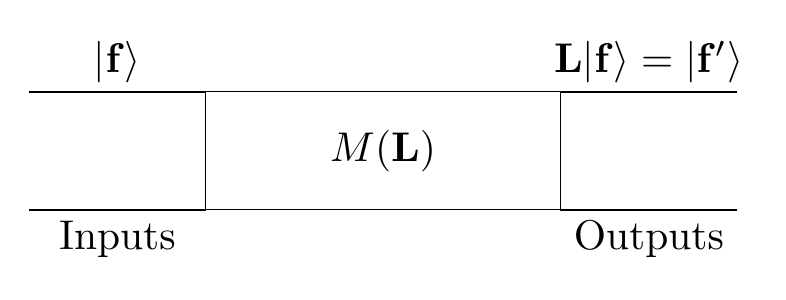
\begin{tikzpicture}[scale=1.5, every node/.style={transform shape}]

% Define coordinates for the main box
\node[draw, minimum width=3cm, minimum height=1cm, align=center] (box) at (0,0) {$M({\bf L})$};

% Inputs line
\draw[thick] (-3, 0.5) -- (-1.5, 0.5);
\draw[thick] (-1.5, -0.5) -- (-3, -0.5);

% Outputs line
\draw[thick] (1.5, 0.5) -- (3, 0.5);
\draw[thick] (1.5, -0.5) -- (3, -0.5);

% Labels for inputs and outputs
\node at (-2.25, 0.75) {$|{\bf f}\rangle$};
\node at (-2.25, -0.75) {Inputs};
\node at (2.25, 0.75) {${\bf L}|{\bf f}\rangle = |{\bf f'}\rangle$};
\node at (2.25, -0.75) {Outputs};

\end{tikzpicture}

\end{document}